\documentclass{article}\usepackage[]{graphicx}\usepackage[]{xcolor}
% maxwidth is the original width if it is less than linewidth
% otherwise use linewidth (to make sure the graphics do not exceed the margin)
\makeatletter
\def\maxwidth{ %
  \ifdim\Gin@nat@width>\linewidth
    \linewidth
  \else
    \Gin@nat@width
  \fi
}
\makeatother

\definecolor{fgcolor}{rgb}{0.345, 0.345, 0.345}
\newcommand{\hlnum}[1]{\textcolor[rgb]{0.686,0.059,0.569}{#1}}%
\newcommand{\hlsng}[1]{\textcolor[rgb]{0.192,0.494,0.8}{#1}}%
\newcommand{\hlcom}[1]{\textcolor[rgb]{0.678,0.584,0.686}{\textit{#1}}}%
\newcommand{\hlopt}[1]{\textcolor[rgb]{0,0,0}{#1}}%
\newcommand{\hldef}[1]{\textcolor[rgb]{0.345,0.345,0.345}{#1}}%
\newcommand{\hlkwa}[1]{\textcolor[rgb]{0.161,0.373,0.58}{\textbf{#1}}}%
\newcommand{\hlkwb}[1]{\textcolor[rgb]{0.69,0.353,0.396}{#1}}%
\newcommand{\hlkwc}[1]{\textcolor[rgb]{0.333,0.667,0.333}{#1}}%
\newcommand{\hlkwd}[1]{\textcolor[rgb]{0.737,0.353,0.396}{\textbf{#1}}}%
\let\hlipl\hlkwb

\usepackage{framed}
\makeatletter
\newenvironment{kframe}{%
 \def\at@end@of@kframe{}%
 \ifinner\ifhmode%
  \def\at@end@of@kframe{\end{minipage}}%
  \begin{minipage}{\columnwidth}%
 \fi\fi%
 \def\FrameCommand##1{\hskip\@totalleftmargin \hskip-\fboxsep
 \colorbox{shadecolor}{##1}\hskip-\fboxsep
     % There is no \\@totalrightmargin, so:
     \hskip-\linewidth \hskip-\@totalleftmargin \hskip\columnwidth}%
 \MakeFramed {\advance\hsize-\width
   \@totalleftmargin\z@ \linewidth\hsize
   \@setminipage}}%
 {\par\unskip\endMakeFramed%
 \at@end@of@kframe}
\makeatother

\definecolor{shadecolor}{rgb}{.97, .97, .97}
\definecolor{messagecolor}{rgb}{0, 0, 0}
\definecolor{warningcolor}{rgb}{1, 0, 1}
\definecolor{errorcolor}{rgb}{1, 0, 0}
\newenvironment{knitrout}{}{} % an empty environment to be redefined in TeX

\usepackage{alltt}
\usepackage[margin=1.0in]{geometry} % To set margins
\usepackage{amsmath}  % This allows me to use the align functionality.
                      % If you find yourself trying to replicate
                      % something you found online, ensure you're
                      % loading the necessary packages!
\usepackage{amsfonts} % Math font
\usepackage{fancyvrb}
\usepackage{hyperref} % For including hyperlinks
\usepackage[shortlabels]{enumitem}% For enumerated lists with labels specified
                    % We had to run tlmgr_install("enumitem") in R
\usepackage{float}    % For telling R where to put a table/figure
\usepackage{natbib}        %For the bibliography
\usepackage[skins,breakable]{tcolorbox}        %For the bibliography
\bibliographystyle{apalike}%For the bibliography
\IfFileExists{upquote.sty}{\usepackage{upquote}}{}
\begin{document}
\noindent\textbf{Homework 7: Robust Regression}\\
\noindent\makebox[\linewidth]{\rule{\textwidth}{0.4pt}}
\noindent\underline{Submission Notes:} Please write your answers to each 
question under that question (not altogether at the end). It will be easier for 
me to give full credit if your answer is commented well, including comments 
about where you are completing each sub-part of the question. For an example,
see Homework 1.\\
\noindent\makebox[\linewidth]{\rule{\textwidth}{0.4pt}}


\begin{enumerate}
  %%%%%%%%%%%%%%%%%%%%%%%%%%%%%%%%%%%%%%%%%%%%%%%%%%%%%%%%%%%%%%%%%%%%%%%%%%%%%%
  %%%%%%%%%%%%%%%%%%%%%%%%%%%%%%%%%%%%%%%%%%%%%%%%%%%%%%%%%%%%%%%%%%%%%%%%%%%%%%
  % Question 1
  %%%%%%%%%%%%%%%%%%%%%%%%%%%%%%%%%%%%%%%%%%%%%%%%%%%%%%%%%%%%%%%%%%%%%%%%%%%%%%
  %%%%%%%%%%%%%%%%%%%%%%%%%%%%%%%%%%%%%%%%%%%%%%%%%%%%%%%%%%%%%%%%%%%%%%%%%%%%%%
  \item Below, I simulate data with heteroskedastic error, noting the variance
  is a function of the predictor $x$.
\begin{knitrout}\scriptsize
\definecolor{shadecolor}{rgb}{0.969, 0.969, 0.969}\color{fgcolor}\begin{kframe}
\begin{alltt}
\hlkwd{set.seed}\hldef{(}\hlnum{1933}\hldef{)}
\hldef{x} \hlkwb{<-} \hlnum{1}\hlopt{:}\hlnum{10}
\hldef{(beta0} \hlkwb{<-} \hlkwd{runif}\hldef{(}\hlnum{1}\hldef{,} \hlopt{-}\hlnum{5}\hldef{,} \hlnum{5}\hldef{))}
\end{alltt}
\begin{verbatim}
## [1] 0.08868237
\end{verbatim}
\begin{alltt}
\hldef{(beta1} \hlkwb{<-} \hlkwd{runif}\hldef{(}\hlnum{1}\hldef{,} \hlopt{-}\hlnum{5}\hldef{,} \hlnum{5}\hldef{))}
\end{alltt}
\begin{verbatim}
## [1] -2.116944
\end{verbatim}
\begin{alltt}
\hldef{y} \hlkwb{<-} \hldef{beta0} \hlopt{+} \hldef{beta1} \hlopt{*} \hldef{x} \hlopt{+} \hlkwd{rnorm}\hldef{(}\hlnum{10}\hldef{,} \hlkwc{mean} \hldef{=} \hlnum{0}\hldef{,} \hlkwc{sd} \hldef{= x)}  \hlcom{# Variance is x^2}

\hldef{dat} \hlkwb{<-} \hlkwd{tibble}\hldef{(}\hlkwc{x} \hldef{= x,}
              \hlkwc{y} \hldef{= y)}
\end{alltt}
\end{kframe}
\end{knitrout}
When I fit an OLS model, it doesn't ``pick up" the regression equation.
\begin{knitrout}\scriptsize
\definecolor{shadecolor}{rgb}{0.969, 0.969, 0.969}\color{fgcolor}\begin{kframe}
\begin{alltt}
\hldef{mod.ols} \hlkwb{<-} \hlkwd{lm}\hldef{(y}\hlopt{~}\hldef{x,} \hlkwc{data}\hldef{=dat)}
\hlkwd{summary}\hldef{(mod.ols)}\hlopt{$}\hldef{coefficients}
\end{alltt}
\begin{verbatim}
##               Estimate Std. Error   t value   Pr(>|t|)
## (Intercept) -6.4290175  2.8929497 -2.222305 0.05697684
## x           -0.7669293  0.4662411 -1.644920 0.13860636
\end{verbatim}
\end{kframe}
\end{knitrout}
In Figure \ref{plotq1}, we see that the increased variance almost creates a 
quadratic (if we ignore the observation at $x=10$)
\begin{knitrout}\scriptsize
\definecolor{shadecolor}{rgb}{0.969, 0.969, 0.969}\color{fgcolor}\begin{kframe}
\begin{alltt}
\hlkwd{ggplot}\hldef{(}\hlkwc{data}\hldef{=dat)}\hlopt{+}
  \hlkwd{geom_point}\hldef{(}\hlkwd{aes}\hldef{(}\hlkwc{x}\hldef{=x,} \hlkwc{y}\hldef{=y))}\hlopt{+}
  \hlkwd{theme_bw}\hldef{()} \hlopt{+}
  \hlkwd{geom_abline}\hldef{(}\hlkwd{aes}\hldef{(}\hlkwc{intercept}\hldef{=}\hlkwd{coef}\hldef{(mod.ols)[}\hlnum{1}\hldef{],}
                  \hlkwc{slope}\hldef{=}\hlkwd{coef}\hldef{(mod.ols)[}\hlnum{2}\hldef{],}
                  \hlkwc{color}\hldef{=}\hlsng{"OLS"}\hldef{))}\hlopt{+}
  \hlkwd{geom_abline}\hldef{(}\hlkwd{aes}\hldef{(}\hlkwc{intercept}\hldef{=beta0,}
                  \hlkwc{slope}\hldef{=beta1,}
                  \hlkwc{color}\hldef{=}\hlsng{"Truth"}\hldef{))}\hlopt{+}
  \hlkwd{labs}\hldef{(}\hlkwc{color}\hldef{=}\hlsng{""}\hldef{)}
\end{alltt}
\end{kframe}
\end{knitrout}
\begin{figure}[H]
\centering
\begin{knitrout}
\definecolor{shadecolor}{rgb}{0.969, 0.969, 0.969}\color{fgcolor}

\includegraphics[width=\maxwidth]{figure/unnamed-chunk-4-1} 
\end{knitrout}
\caption{Heteroskedastic regression data generated for Question 1.}\label{plotq1}
\end{figure}
\begin{enumerate}
  \item Conduct a residual and influence analysis on the \texttt{mod.ols}.\\
  \textbf{Note:} The \emph{known} issue may not be obvious.
  
  \begin{figure}[H]
  \centering
  
\begin{knitrout}\scriptsize
\definecolor{shadecolor}{rgb}{0.969, 0.969, 0.969}\color{fgcolor}\begin{kframe}
\begin{alltt}
\hlkwd{source}\hldef{(}\hlsng{"plotResiduals.R"}\hldef{)}
\hlkwd{source}\hldef{(}\hlsng{"plotInfluence.R"}\hldef{)}

\hlkwd{plotResiduals}\hldef{(mod.ols)}
\end{alltt}
\end{kframe}

\includegraphics[width=\maxwidth]{figure/unnamed-chunk-5-1} 
\end{knitrout}
  
  \label{residual.mod}
  \caption{Residual Analysis on \texttt{mod.ols}}
  \end{figure}
  
  \textcolor{red}{If I was analyzing the residuals of this model I would assume there was a non-linear relationship between the predictors and the response variable due to the clear curved pattern in the residuals. The histogram of the residuals looks a little skewed but it's not terrible for 10 observations. The qqplot indicates a potential non-linear relationship with the quadratic looking pattern on the right tail.}
  
  \begin{figure}[H]
  \centering
  
\begin{knitrout}\scriptsize
\definecolor{shadecolor}{rgb}{0.969, 0.969, 0.969}\color{fgcolor}\begin{kframe}
\begin{alltt}
\hlkwd{plotInfluence}\hldef{(mod.ols)}
\end{alltt}
\end{kframe}

\includegraphics[width=\maxwidth]{figure/unnamed-chunk-6-1} 
\end{knitrout}
  
  \label{influence.mod}
  \caption{Influence Analysis on \texttt{mod.ols}}
  \end{figure}
  
  \textcolor{red}{Looking at the influence, the thing that stands out is the clear leverage pattern across observation numbers, which would indicate to me that the observations are not independent of each other. The studentized residuals show similar problems to the residuals in Figure: \ref{influence.mod}. Additionally, with there only being 10 observations, several of them having large Cook's d and DFFITs is a bit concerning due to the sheer proportion of potentially high influence points making up a large part of the model.}
  
  \item Fit a weighted least squares (WLS) regression model.
  \begin{enumerate}
    \item Why is $w_i = 1/x_i^2$ a sensible choice for the weights?\\
    \textbf{Hint:} Why is the RMSE $\approx 1$?

\textcolor{red}{In the setup of the regression equation the variance at each point $x$(1:10) is $x^2$, so weighting each point by $\frac{1}{x^2}$ should make each point have weighted variance 1.}

    
    \item Fit the model with these weights, how does the result change?
    
\begin{knitrout}\scriptsize
\definecolor{shadecolor}{rgb}{0.969, 0.969, 0.969}\color{fgcolor}\begin{kframe}
\begin{alltt}
\hldef{weights} \hlkwb{=} \hlnum{1}\hlopt{/}\hldef{x}\hlopt{^}\hlnum{2}

\hldef{mod_weighted} \hlkwb{<-} \hlkwd{lm}\hldef{(y} \hlopt{~} \hldef{x,} \hlkwc{data} \hldef{= dat,} \hlkwc{weights} \hldef{= weights)}

\hldef{(sum} \hlkwb{<-} \hlkwd{summary}\hldef{(mod_weighted))}
\end{alltt}
\begin{verbatim}
## 
## Call:
## lm(formula = y ~ x, data = dat, weights = weights)
## 
## Weighted Residuals:
##     Min      1Q  Median      3Q     Max 
## -2.0210 -0.6560  0.0217  0.7014  1.4473 
## 
## Coefficients:
##             Estimate Std. Error t value Pr(>|t|)   
## (Intercept)  -1.7035     1.3762  -1.238  0.25088   
## x            -1.8698     0.5418  -3.451  0.00868 **
## ---
## Signif. codes:  0 '***' 0.001 '**' 0.01 '*' 0.05 '.' 0.1 ' ' 1
## 
## Residual standard error: 1.145 on 8 degrees of freedom
## Multiple R-squared:  0.5982,	Adjusted R-squared:  0.548 
## F-statistic: 11.91 on 1 and 8 DF,  p-value: 0.008678
\end{verbatim}
\end{kframe}
\end{knitrout}
 
 \textcolor{red}{Now that we used the weighted model, the coefficent $\beta_1$ associated with $x$ is estimated to be -1.8698 ($p = 0.00868$). This is only a few tenths greater than the true value of $\beta_1 = -2.1169$. The intercept $\beta_0$ is estimated to be -1.7035 while the true $\beta_0$ is 0.0887, indicating that the estimate for the intercept is still quite off. This would probably be better if the data extended more for $x \leq 0$.}
    
    \item Add the WLS line to the scatterplot.
    
    \begin{figure}[H]
    \centering
    
\begin{knitrout}\scriptsize
\definecolor{shadecolor}{rgb}{0.969, 0.969, 0.969}\color{fgcolor}\begin{kframe}
\begin{alltt}
\hldef{betas} \hlkwb{<-} \hldef{sum}\hlopt{$}\hldef{coefficients}
\hldef{beta0_w} \hlkwb{<-} \hldef{betas[}\hlnum{1}\hldef{,}\hlnum{1}\hldef{]}
\hldef{beta1_w} \hlkwb{<-} \hldef{betas[}\hlnum{2}\hldef{,}\hlnum{1}\hldef{]}

\hlkwd{ggplot}\hldef{(}\hlkwc{data}\hldef{=dat)}\hlopt{+}
  \hlkwd{geom_point}\hldef{(}\hlkwd{aes}\hldef{(}\hlkwc{x}\hldef{=x,} \hlkwc{y}\hldef{=y))}\hlopt{+}
  \hlkwd{theme_bw}\hldef{()} \hlopt{+}
  \hlkwd{geom_abline}\hldef{(}\hlkwd{aes}\hldef{(}\hlkwc{intercept}\hldef{=}\hlkwd{coef}\hldef{(mod.ols)[}\hlnum{1}\hldef{],}
              \hlkwc{slope}\hldef{=}\hlkwd{coef}\hldef{(mod.ols)[}\hlnum{2}\hldef{],}
              \hlkwc{color}\hldef{=}\hlsng{"OLS"}\hldef{))}\hlopt{+}
  \hlkwd{geom_abline}\hldef{(}\hlkwd{aes}\hldef{(}\hlkwc{intercept}\hldef{=beta0,}
              \hlkwc{slope}\hldef{=beta1,}
              \hlkwc{color}\hldef{=}\hlsng{"Truth"}\hldef{))}\hlopt{+}
  \hlkwd{geom_abline}\hldef{(}\hlkwd{aes}\hldef{(}\hlkwc{intercept} \hldef{= beta0_w,}
              \hlkwc{slope}\hldef{=beta1_w,}
              \hlkwc{color}\hldef{=}\hlsng{"WLS"}\hldef{))} \hlopt{+}
  \hlkwd{labs}\hldef{(}\hlkwc{color}\hldef{=}\hlsng{""}\hldef{)} \hlopt{+}
  \hlkwd{geom_hline}\hldef{(}\hlkwc{yintercept} \hldef{=} \hlnum{0}\hldef{,} \hlkwc{linetype}\hldef{=}\hlsng{"dashed"}\hldef{)}
\end{alltt}
\end{kframe}

\includegraphics[width=\maxwidth]{figure/unnamed-chunk-8-1} 
\end{knitrout}
    
    \label{new.mod}
    \caption{Scatterplot with Estimated Regression Lines (Updated With Weighted OLS Model)}
    
    \end{figure}
    
    \textcolor{red}{The weighted model worked as intended here, as clearly the WLS regression line is much closer to the truth than the OLS regression line.}
    
  \end{enumerate}
\end{enumerate}
  %%%%%%%%%%%%%%%%%%%%%%%%%%%%%%%%%%%%%%%%%%%%%%%%%%%%%%%%%%%%%%%%%%%%%%%%%%%%%%
  %%%%%%%%%%%%%%%%%%%%%%%%%%%%%%%%%%%%%%%%%%%%%%%%%%%%%%%%%%%%%%%%%%%%%%%%%%%%%%
  % Question 2
  %%%%%%%%%%%%%%%%%%%%%%%%%%%%%%%%%%%%%%%%%%%%%%%%%%%%%%%%%%%%%%%%%%%%%%%%%%%%%%
  %%%%%%%%%%%%%%%%%%%%%%%%%%%%%%%%%%%%%%%%%%%%%%%%%%%%%%%%%%%%%%%%%%%%%%%%%%%%%%
\item Explore fitting a regression model to the data simulated below.
\begin{knitrout}\scriptsize
\definecolor{shadecolor}{rgb}{0.969, 0.969, 0.969}\color{fgcolor}\begin{kframe}
\begin{alltt}
\hldef{n} \hlkwb{<-} \hlnum{50}
\hlkwd{set.seed}\hldef{(}\hlnum{7272}\hldef{)}
\hldef{x} \hlkwb{<-} \hlkwd{sample}\hldef{(}\hlkwc{x}\hldef{=}\hlkwd{seq}\hldef{(}\hlnum{0}\hldef{,}\hlnum{100}\hldef{,}\hlnum{0.01}\hldef{),} \hlkwc{size}\hldef{=n,} \hlkwc{replace}\hldef{=}\hlnum{TRUE}\hldef{)}
\hldef{e} \hlkwb{<-} \hlkwd{rnorm}\hldef{(}\hlkwc{n}\hldef{=}\hlnum{50}\hldef{,} \hlkwc{mean}\hldef{=}\hlnum{0}\hldef{,} \hlkwc{sd}\hldef{=}\hlnum{5}\hldef{)}
\hldef{y} \hlkwb{<-} \hlnum{3.5} \hlopt{+} \hlnum{2.1}\hlopt{*}\hldef{x} \hlopt{+} \hldef{e}

\hldef{first_dat} \hlkwb{<-} \hlkwd{tibble}\hldef{(}\hlkwc{x} \hldef{= x,}
                    \hlkwc{y} \hldef{= y)}

\hlcom{# Add a misbehaved point}
\hldef{x2} \hlkwb{<-} \hlkwd{c}\hldef{(x,} \hlnum{100}\hldef{)}
\hldef{y2} \hlkwb{<-} \hlkwd{c}\hldef{(y,} \hlnum{25}\hldef{)}
\end{alltt}
\end{kframe}
\end{knitrout}
\begin{enumerate}
	\item Fit an OLS model based on \texttt{x} and \texttt{y}. Check the assumptions of the model and interpret the 
	coefficients of the model; are they what you would expect?
	
\begin{knitrout}\scriptsize
\definecolor{shadecolor}{rgb}{0.969, 0.969, 0.969}\color{fgcolor}\begin{kframe}
\begin{alltt}
\hldef{first_mod} \hlkwb{<-} \hlkwd{lm}\hldef{(y} \hlopt{~} \hldef{x,} \hlkwc{data} \hldef{= first_dat)}
\end{alltt}
\end{kframe}
\end{knitrout}
	
	\begin{figure}[H]
	\centering
	
\begin{knitrout}\scriptsize
\definecolor{shadecolor}{rgb}{0.969, 0.969, 0.969}\color{fgcolor}\begin{kframe}
\begin{alltt}
\hldef{first_mod} \hlkwb{<-} \hlkwd{lm}\hldef{(y} \hlopt{~} \hldef{x,} \hlkwc{data} \hldef{= first_dat)}

\hlkwd{plotResiduals}\hldef{(first_mod)}
\end{alltt}
\end{kframe}

\includegraphics[width=\maxwidth]{figure/unnamed-chunk-11-1} 
\end{knitrout}
	
	\label{first.mod.residual}
	\caption{Residual Analysis on \texttt{x} and \texttt{y} OLS model}
	\end{figure}
	
	\textcolor{red}{The residuals look perfect. They're centered at 0 with good normality. The qqplot is very reasonable. Finally, the residuals are indiscriminantly scattered with constant variance.}
	
	\begin{figure}[H]
	\centering
	
\begin{knitrout}\scriptsize
\definecolor{shadecolor}{rgb}{0.969, 0.969, 0.969}\color{fgcolor}\begin{kframe}
\begin{alltt}
\hlkwd{plotInfluence}\hldef{(first_mod)}
\end{alltt}
\end{kframe}
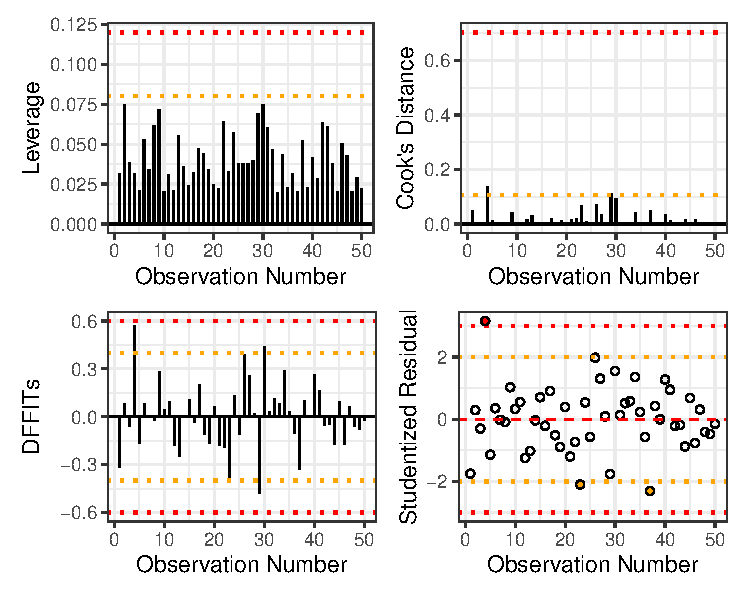
\includegraphics[width=\maxwidth]{figure/unnamed-chunk-12-1} 
\end{knitrout}
	
	\label{first.mod.influence}
	\caption{Influence Analysis on \texttt{x} and \texttt{y} OLS model}
	\end{figure}
	
	\item Fit an OLS model based on \texttt{x2} and \texttt{y2}. Check the assumptions of the model and interpret the 
	coefficients of the model; are they what you would expect?
\end{enumerate}
  %%%%%%%%%%%%%%%%%%%%%%%%%%%%%%%%%%%%%%%%%%%%%%%%%%%%%%%%%%%%%%%%%%%%%%%%%%%%%%
  %%%%%%%%%%%%%%%%%%%%%%%%%%%%%%%%%%%%%%%%%%%%%%%%%%%%%%%%%%%%%%%%%%%%%%%%%%%%%%
  % Question 3
  %%%%%%%%%%%%%%%%%%%%%%%%%%%%%%%%%%%%%%%%%%%%%%%%%%%%%%%%%%%%%%%%%%%%%%%%%%%%%%
  %%%%%%%%%%%%%%%%%%%%%%%%%%%%%%%%%%%%%%%%%%%%%%%%%%%%%%%%%%%%%%%%%%%%%%%%%%%%%%
\item Continue with Question 2.
\begin{enumerate}
  \item Fit an IRWLS model based on \texttt{x2} and \texttt{y2} using Huber 
  weights. Interpret the coefficients of the model; are they what you would expect?
  \item Fit an IRWLS model based on \texttt{x2} and \texttt{y2} using Bisquare 
  weights. Interpret the coefficients of the model; are they what you would expect?
  \item Fit an IRWLS model based on \texttt{x2} and \texttt{y2} using \texttt{lmrob()} 
  from the \texttt{robustbase} package for \texttt{R}. Interpret the coefficients 
  of the model; are they what you would expect?
  \item Fit a Quantile regression model based on \texttt{x2} and \texttt{y2}.
  Interpret the coefficients of the model; are they what you would expect?
\end{enumerate}
  %%%%%%%%%%%%%%%%%%%%%%%%%%%%%%%%%%%%%%%%%%%%%%%%%%%%%%%%%%%%%%%%%%%%%%%%%%%%%%
  %%%%%%%%%%%%%%%%%%%%%%%%%%%%%%%%%%%%%%%%%%%%%%%%%%%%%%%%%%%%%%%%%%%%%%%%%%%%%%
  % Question 4
  %%%%%%%%%%%%%%%%%%%%%%%%%%%%%%%%%%%%%%%%%%%%%%%%%%%%%%%%%%%%%%%%%%%%%%%%%%%%%%
  %%%%%%%%%%%%%%%%%%%%%%%%%%%%%%%%%%%%%%%%%%%%%%%%%%%%%%%%%%%%%%%%%%%%%%%%%%%%%%
\item \textbf{Optional, but recommended} Plot the results! Create a scatterplot
of \texttt{x2} and \texttt{y2}. Superimpose the true regression line, the OLS
estimate, the IRWLS estimates, and the quantile regression estimate. Interpret
the results.
  %%%%%%%%%%%%%%%%%%%%%%%%%%%%%%%%%%%%%%%%%%%%%%%%%%%%%%%%%%%%%%%%%%%%%%%%%%%%%%
  %%%%%%%%%%%%%%%%%%%%%%%%%%%%%%%%%%%%%%%%%%%%%%%%%%%%%%%%%%%%%%%%%%%%%%%%%%%%%%
  % Question 5
  %%%%%%%%%%%%%%%%%%%%%%%%%%%%%%%%%%%%%%%%%%%%%%%%%%%%%%%%%%%%%%%%%%%%%%%%%%%%%%
  %%%%%%%%%%%%%%%%%%%%%%%%%%%%%%%%%%%%%%%%%%%%%%%%%%%%%%%%%%%%%%%%%%%%%%%%%%%%%%
\item \textbf{Optional, but recommended} Complete Questions 3-4, but use $n=1000$.
What changes? Why do you think that is?

\end{enumerate}
\bibliography{bib}
\end{document}

